\documentclass[graphics]{beamer}
\usepackage{graphicx}
\usepackage{listings} % Syntax highlighing
\usepackage{fancyvrb} % Inline verbatim
\usepackage{hyperref} % Hyperlinks
\hypersetup{pdfpagemode=FullScreen}

\usepackage[normalem]{ulem}               % to striketrhourhg text
\newcommand\redout{\bgroup\markoverwith
{\textcolor{red}{\rule[0.5ex]{2pt}{0.8pt}}}\ULon}

% header in tables
\newcommand*{\thead}[1]{\multicolumn{1}{c}{\bfseries #1}}

% used for arrows from one point in the slide to another
\usepackage{tikz}
\usetikzlibrary{arrows,shapes,tikzmark}

\usetheme{Boadilla}
\title{Lecture 7: Variables in C}
\author{UMBC CMSC 104}
\date{Th 23 Sept 2021}

\begin{document}

\begin{frame}{}
\centering
    Variables in C
\end{frame}

\begin{frame}{Variables in C}
    Topics:
    \begin{itemize}
        \item Naming Variables
        \item Declaring Variables
        \item Using Variables
        \item The Assignment Statement
    \end{itemize}
\end{frame}

\begin{frame}{What Are Variables in C?}
    \begin{itemize}
        \item \textbf{Variables} in C have the same meaning as variables in algebra. That is, they represent some unknown, or variable, value. \\
        \centering{
        $x = a + b$ \\
        $x + 2 = 3(y-5)$}
        \item Remember that variables in algebra are represented by a single alphabetic character. In C, that's not usually the case.
    \end{itemize}
\end{frame}

\section*{Naming Variables}
\begin{frame}{Legal Identifiers in C}
    \begin{itemize}
        \item Another name for a variable in C is an identifier.
        \item Variables in C may be given representations containing multiple characters, but there are rules for these representations.
        \item Legal or valid variable names in C:
        \begin{itemize}
            \item May only consist of letters, digits, and underscores.
            \item May be as long as you like, but only the first 31 characters are significant.
            \item May not begin with a number.
            \item May not be a C \textbf{reserved word (keyword)}.
        \end{itemize}
    \end{itemize}
\end{frame}

\begin{frame}{Reserved Words (Keywords) in C}
    \centering
    \begin{tabular}{l l l l}
        auto   & break     & int      & long   \\ [5pt]
        case    & char     & register & return \\ [5pt]
        const   & continue & short    & signed \\ [5pt]
        default & do       & sizeof   & static \\ [5pt]
        double  & else     & struct   & switch \\ [5pt]
        enum    & extern   & typedef  & union  \\ [5pt]
        float   & for      & unsigned & void   \\ [5pt]
        goto    & if       & volatile & while
    \end{tabular}
\end{frame}

\begin{frame}{CMSC104 Naming Conventions}
    C programmers generally agree on the following \textbf{conventions} for naming variables:
    \begin{itemize}
        \item Begin variable names with lowercase letters.
        \item Use meaningful identifiers (name)
        \item Separate ``words'' within identifiers with underscores or mixed upper and lower case. \\
        ~~ ~~ Example: surfaceArea, surface\_area, surface\_Area
        \item Be consistent!
    \end{itemize}
\end{frame}

\begin{frame}{Case Sensitivity}
    C is \textbf{case sensitive}
    \begin{itemize}
        \item It matters whether a variable name is uppercase or lowercase.
        \item These are all different: \\
        ~~ ~~ area \\
        ~~ ~~ Area \\
        ~~ ~~ AREA \\
        ~~ ~~ ArEa
    \end{itemize}
\end{frame}

\begin{frame}{Legal Identifiers vs. Naming Conventions}
    \begin{itemize}
        \item \textbf{Legal identifiers} refer to the restrictions C places on naming identifiers, such as not beginning with a number.
        \item \textbf{Naming conventions} refer to the standards you must follow for this course, such as all variable names must be lowercase. But this isn't technically required by the compiler.
    \end{itemize}
\end{frame}

\begin{frame}{Which are Legal Identifiers?}
    \centering
    \only<1> {
        \begin{tabular}{l l}
            AREA & 3D \\ [5pt]
            lucky*** & num45 \\ [5pt]
            Last-Chance & \#values \\ [5pt]
            x\_yt3 & pi \\ [5pt]
            num\$ & \%done \\ [5pt]
            area\_under\_the\_curve
        \end{tabular}
    }
    \only<2> {
        \begin{tabular}{l l}
            AREA & \sout{3D} \\ [5pt]
            \sout{lucky***} & num45 \\ [5pt]
            \sout{Last-Chance} & \sout{\#values} \\ [5pt]
            x\_yt3 & pi \\ [5pt]
            \sout{num\$} & \sout{\%done} \\ [5pt]
            area\_under\_the\_curve
        \end{tabular}
    }
    \only<3> {
        Why? \hfil
        \begin{itemize}
            \item * means something specific, which we'll get to later.
            \item How is the compiler supposed to know the difference between the hyphen in a variable name vs. subtraction?
            \item \%, \$, \#, \$, (, ), {, }, etc are not allowed to be in a variable name.
        \end{itemize}
    }
\end{frame}

\begin{frame}{Which Follow the CMSC104 Naming Conventions?}
    \centering
    \only<1> {
        \begin{tabular}{l l}
            Area & person1 \\ [5pt]
            Last\_Chance & values \\ [5pt]
            x\_yt3 & pi \\ [5pt]
            finaltotal & numChildren \\ [5pt]
            area\_under\_the\_curve
        \end{tabular}
    }
    \only<2> {
        \begin{tabular}{l l}
            \sout{Area} & person1 \\ [5pt]
            \sout{Last\_Chance} & values \\ [5pt]
            x\_yt3 & pi \\ [5pt]
            \sout{finaltotal} & numChildren \\ [5pt]
            area\_under\_the\_curve
        \end{tabular}
    }
\end{frame}

\section*{Declaring Variables}
\begin{frame}{Declaring Variables}
    \only<1> {
        \begin{itemize}
            \item Before using a variable, you must give the compiler some information about the variable. You must \textbf{declare} it.
            \item The \textbf{declaration statement} includes the \textbf{data type} of the variable.
            \item Examples: \\
            ~~ ~~ int meatballs; \\
            ~~ ~~ float area;
        \end{itemize}
    }
    \only<2> {
        When we declare a variable:
        \begin{itemize}
            \item Space in RAM is set aside to hold a value of the specified \textbf{data type}.
            \item That space is associated with the variable \textbf{name}.
            \item That space is associated with a unique \textbf{address}.
        \end{itemize}
        % Graphic for TeX using PGF
% Title: /home/rjzak/Desktop/cmsc104/L07_declaring.dia
% Creator: Dia v0.97+git
% CreationDate: Wed Sep 22 22:29:43 2021
% For: rjzak
% \usepackage{tikz}
% The following commands are not supported in PSTricks at present
% We define them conditionally, so when they are implemented,
% this pgf file will use them.
\ifx\du\undefined
  \newlength{\du}
\fi
\setlength{\du}{15\unitlength}
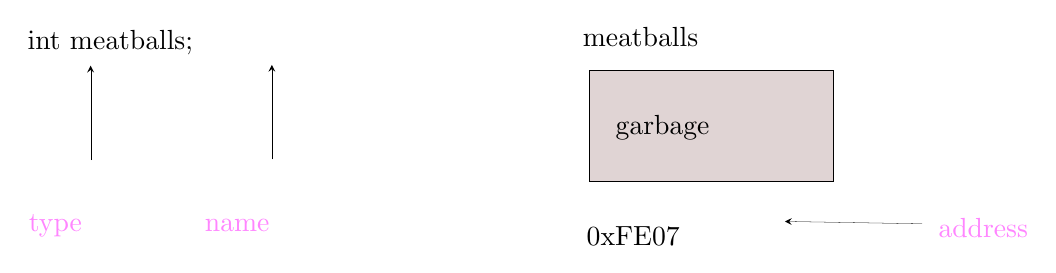
\begin{tikzpicture}[even odd rule]
\pgftransformxscale{1.000000}
\pgftransformyscale{-1.000000}
\definecolor{dialinecolor}{rgb}{0.000000, 0.000000, 0.000000}
\pgfsetstrokecolor{dialinecolor}
\pgfsetstrokeopacity{1.000000}
\definecolor{diafillcolor}{rgb}{1.000000, 1.000000, 1.000000}
\pgfsetfillcolor{diafillcolor}
\pgfsetfillopacity{1.000000}
% setfont left to latex
\definecolor{dialinecolor}{rgb}{0.000000, 0.000000, 0.000000}
\pgfsetstrokecolor{dialinecolor}
\pgfsetstrokeopacity{1.000000}
\definecolor{diafillcolor}{rgb}{0.000000, 0.000000, 0.000000}
\pgfsetfillcolor{diafillcolor}
\pgfsetfillopacity{1.000000}
\node[anchor=base west,inner sep=0pt,outer sep=0pt,color=dialinecolor] at (1.900000\du,3.450000\du){int meatballs;};
% setfont left to latex
\definecolor{dialinecolor}{rgb}{1.000000, 0.521569, 1.000000}
\pgfsetstrokecolor{dialinecolor}
\pgfsetstrokeopacity{1.000000}
\definecolor{diafillcolor}{rgb}{1.000000, 0.521569, 1.000000}
\pgfsetfillcolor{diafillcolor}
\pgfsetfillopacity{1.000000}
\node[anchor=base west,inner sep=0pt,outer sep=0pt,color=dialinecolor] at (1.916667\du,5.750000\du){type};
% setfont left to latex
\definecolor{dialinecolor}{rgb}{1.000000, 0.521569, 1.000000}
\pgfsetstrokecolor{dialinecolor}
\pgfsetstrokeopacity{1.000000}
\definecolor{diafillcolor}{rgb}{1.000000, 0.521569, 1.000000}
\pgfsetfillcolor{diafillcolor}
\pgfsetfillopacity{1.000000}
\node[anchor=base west,inner sep=0pt,outer sep=0pt,color=dialinecolor] at (4.150000\du,5.750000\du){name};
\pgfsetlinewidth{0.100000\du}
\pgfsetdash{}{0pt}
\pgfsetbuttcap
{
\definecolor{diafillcolor}{rgb}{0.000000, 0.000000, 0.000000}
\pgfsetfillcolor{diafillcolor}
\pgfsetfillopacity{1.000000}
% was here!!!
\pgfsetarrowsend{stealth}
\definecolor{dialinecolor}{rgb}{0.000000, 0.000000, 0.000000}
\pgfsetstrokecolor{dialinecolor}
\pgfsetstrokeopacity{1.000000}
\draw (2.700000\du,4.850000\du)--(2.700000\du,3.650000\du);
}
\pgfsetlinewidth{0.100000\du}
\pgfsetdash{}{0pt}
\pgfsetbuttcap
{
\definecolor{diafillcolor}{rgb}{0.000000, 0.000000, 0.000000}
\pgfsetfillcolor{diafillcolor}
\pgfsetfillopacity{1.000000}
% was here!!!
\pgfsetarrowsend{stealth}
\definecolor{dialinecolor}{rgb}{0.000000, 0.000000, 0.000000}
\pgfsetstrokecolor{dialinecolor}
\pgfsetstrokeopacity{1.000000}
\draw (5.001803\du,4.840000\du)--(5.001803\du,3.640000\du);
}
% setfont left to latex
\definecolor{dialinecolor}{rgb}{0.000000, 0.000000, 0.000000}
\pgfsetstrokecolor{dialinecolor}
\pgfsetstrokeopacity{1.000000}
\definecolor{diafillcolor}{rgb}{0.000000, 0.000000, 0.000000}
\pgfsetfillcolor{diafillcolor}
\pgfsetfillopacity{1.000000}
\node[anchor=base west,inner sep=0pt,outer sep=0pt,color=dialinecolor] at (8.950000\du,3.411767\du){meatballs};
\pgfsetlinewidth{0.020000\du}
\pgfsetdash{}{0pt}
\pgfsetmiterjoin
\pgfsetbuttcap
{\pgfsetcornersarced{\pgfpoint{0.000000\du}{0.000000\du}}\definecolor{diafillcolor}{rgb}{0.878431, 0.831373, 0.831373}
\pgfsetfillcolor{diafillcolor}
\pgfsetfillopacity{1.000000}
\fill (9.033333\du,3.711767\du)--(9.033333\du,5.111767\du)--(12.133333\du,5.111767\du)--(12.133333\du,3.711767\du)--cycle;
}{\pgfsetcornersarced{\pgfpoint{0.000000\du}{0.000000\du}}\definecolor{dialinecolor}{rgb}{0.000000, 0.000000, 0.000000}
\pgfsetstrokecolor{dialinecolor}
\pgfsetstrokeopacity{1.000000}
\draw (9.033333\du,3.711767\du)--(9.033333\du,5.111767\du)--(12.133333\du,5.111767\du)--(12.133333\du,3.711767\du)--cycle;
}% setfont left to latex
\definecolor{dialinecolor}{rgb}{0.000000, 0.000000, 0.000000}
\pgfsetstrokecolor{dialinecolor}
\pgfsetstrokeopacity{1.000000}
\definecolor{diafillcolor}{rgb}{0.000000, 0.000000, 0.000000}
\pgfsetfillcolor{diafillcolor}
\pgfsetfillopacity{1.000000}
\node[anchor=base west,inner sep=0pt,outer sep=0pt,color=dialinecolor] at (9.366667\du,4.528433\du){garbage};
% setfont left to latex
\definecolor{dialinecolor}{rgb}{0.000000, 0.000000, 0.000000}
\pgfsetstrokecolor{dialinecolor}
\pgfsetstrokeopacity{1.000000}
\definecolor{diafillcolor}{rgb}{0.000000, 0.000000, 0.000000}
\pgfsetfillcolor{diafillcolor}
\pgfsetfillopacity{1.000000}
\node[anchor=base west,inner sep=0pt,outer sep=0pt,color=dialinecolor] at (9.000000\du,5.928433\du){0xFE07};
% setfont left to latex
\definecolor{dialinecolor}{rgb}{1.000000, 0.521569, 1.000000}
\pgfsetstrokecolor{dialinecolor}
\pgfsetstrokeopacity{1.000000}
\definecolor{diafillcolor}{rgb}{1.000000, 0.521569, 1.000000}
\pgfsetfillcolor{diafillcolor}
\pgfsetfillopacity{1.000000}
\node[anchor=base west,inner sep=0pt,outer sep=0pt,color=dialinecolor] at (13.466667\du,5.828433\du){address};
\pgfsetlinewidth{0.100000\du}
\pgfsetdash{}{0pt}
\pgfsetbuttcap
{
\definecolor{diafillcolor}{rgb}{0.000000, 0.000000, 0.000000}
\pgfsetfillcolor{diafillcolor}
\pgfsetfillopacity{1.000000}
% was here!!!
\pgfsetarrowsend{stealth}
\definecolor{dialinecolor}{rgb}{0.000000, 0.000000, 0.000000}
\pgfsetstrokecolor{dialinecolor}
\pgfsetstrokeopacity{1.000000}
\draw (13.258470\du,5.658433\du)--(11.516667\du,5.628433\du);
}
\end{tikzpicture}

    }
\end{frame}

\begin{frame}{More About Variables}
    C has three basic predefined data types:
    \begin{itemize}
        \item Integers (whole numbers)
        \begin{itemize}
            \item \textbf{int}, long int (or just long), short int (or just short)
            \item Always positive: unsigned (unsigned int, unsigned long, unsigned short)
        \end{itemize}
        \item Floating point (real numbers)
        \begin{itemize}
            \item \textbf{float}, \textbf{double}
        \end{itemize}
        \item Characters
        \begin{itemize}
            \item \textbf{char}
        \end{itemize}
    \end{itemize}
\end{frame}

\section*{Using Variables}
\begin{frame}{Using Variables: Initialization}
    Variables may be given initial values, or \textbf{initialized}, when declared. \\
    % Graphic for TeX using PGF
% Title: /home/rjzak/Desktop/cmsc104/L07_initializing.dia
% Creator: Dia v0.97+git
% CreationDate: Wed Sep 22 22:43:35 2021
% For: rjzak
% \usepackage{tikz}
% The following commands are not supported in PSTricks at present
% We define them conditionally, so when they are implemented,
% this pgf file will use them.
\ifx\du\undefined
  \newlength{\du}
\fi
\setlength{\du}{15\unitlength}
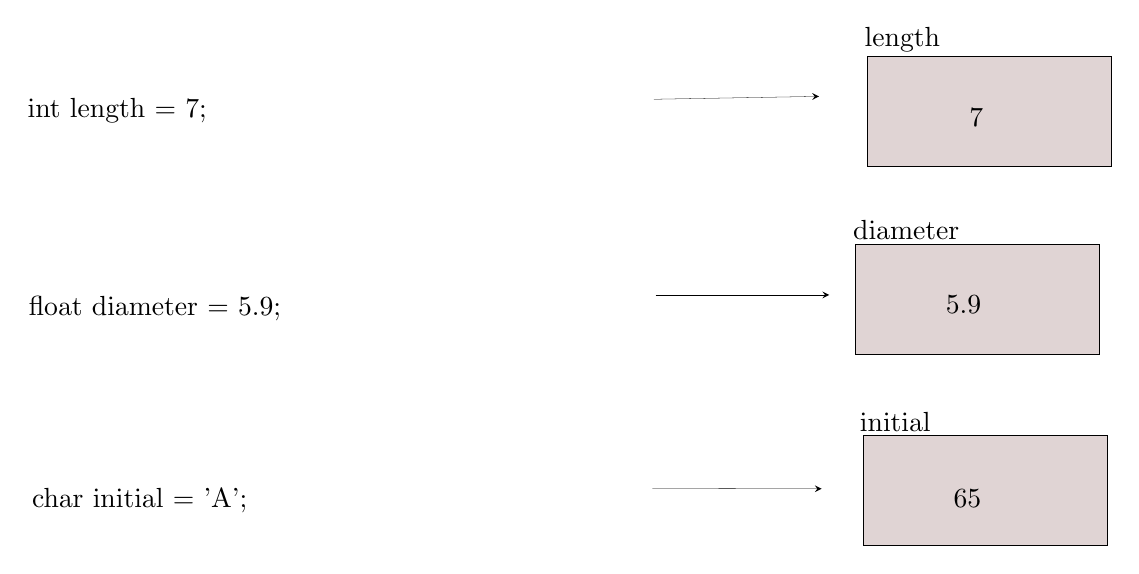
\begin{tikzpicture}[even odd rule]
\pgftransformxscale{1.000000}
\pgftransformyscale{-1.000000}
\definecolor{dialinecolor}{rgb}{0.000000, 0.000000, 0.000000}
\pgfsetstrokecolor{dialinecolor}
\pgfsetstrokeopacity{1.000000}
\definecolor{diafillcolor}{rgb}{1.000000, 1.000000, 1.000000}
\pgfsetfillcolor{diafillcolor}
\pgfsetfillopacity{1.000000}
% setfont left to latex
\definecolor{dialinecolor}{rgb}{0.000000, 0.000000, 0.000000}
\pgfsetstrokecolor{dialinecolor}
\pgfsetstrokeopacity{1.000000}
\definecolor{diafillcolor}{rgb}{0.000000, 0.000000, 0.000000}
\pgfsetfillcolor{diafillcolor}
\pgfsetfillopacity{1.000000}
\node[anchor=base west,inner sep=0pt,outer sep=0pt,color=dialinecolor] at (1.925000\du,3.200000\du){int length = 7;};
\pgfsetlinewidth{0.100000\du}
\pgfsetdash{}{0pt}
\pgfsetbuttcap
{
\definecolor{diafillcolor}{rgb}{0.000000, 0.000000, 0.000000}
\pgfsetfillcolor{diafillcolor}
\pgfsetfillopacity{1.000000}
% was here!!!
\pgfsetarrowsend{stealth}
\definecolor{dialinecolor}{rgb}{0.000000, 0.000000, 0.000000}
\pgfsetstrokecolor{dialinecolor}
\pgfsetstrokeopacity{1.000000}
\draw (9.900000\du,5.450000\du)--(12.105000\du,5.450000\du);
}
\pgfsetlinewidth{0.100000\du}
\pgfsetdash{}{0pt}
\pgfsetbuttcap
{
\definecolor{diafillcolor}{rgb}{0.000000, 0.000000, 0.000000}
\pgfsetfillcolor{diafillcolor}
\pgfsetfillopacity{1.000000}
% was here!!!
\pgfsetarrowsend{stealth}
\definecolor{dialinecolor}{rgb}{0.000000, 0.000000, 0.000000}
\pgfsetstrokecolor{dialinecolor}
\pgfsetstrokeopacity{1.000000}
\draw (9.876800\du,2.965000\du)--(11.975000\du,2.928474\du);
}
\pgfsetlinewidth{0.020000\du}
\pgfsetdash{}{0pt}
\pgfsetmiterjoin
\pgfsetbuttcap
{\pgfsetcornersarced{\pgfpoint{0.000000\du}{0.000000\du}}\definecolor{diafillcolor}{rgb}{0.878431, 0.831373, 0.831373}
\pgfsetfillcolor{diafillcolor}
\pgfsetfillopacity{1.000000}
\fill (12.583330\du,2.411770\du)--(12.583330\du,3.811770\du)--(15.683330\du,3.811770\du)--(15.683330\du,2.411770\du)--cycle;
}{\pgfsetcornersarced{\pgfpoint{0.000000\du}{0.000000\du}}\definecolor{dialinecolor}{rgb}{0.000000, 0.000000, 0.000000}
\pgfsetstrokecolor{dialinecolor}
\pgfsetstrokeopacity{1.000000}
\draw (12.583330\du,2.411770\du)--(12.583330\du,3.811770\du)--(15.683330\du,3.811770\du)--(15.683330\du,2.411770\du)--cycle;
}\pgfsetlinewidth{0.100000\du}
\pgfsetdash{}{0pt}
\pgfsetbuttcap
{
\definecolor{diafillcolor}{rgb}{0.000000, 0.000000, 0.000000}
\pgfsetfillcolor{diafillcolor}
\pgfsetfillopacity{1.000000}
% was here!!!
\pgfsetarrowsend{stealth}
\definecolor{dialinecolor}{rgb}{0.000000, 0.000000, 0.000000}
\pgfsetstrokecolor{dialinecolor}
\pgfsetstrokeopacity{1.000000}
\draw (9.858500\du,7.908430\du)--(12.008333\du,7.911807\du);
}
% setfont left to latex
\definecolor{dialinecolor}{rgb}{0.000000, 0.000000, 0.000000}
\pgfsetstrokecolor{dialinecolor}
\pgfsetstrokeopacity{1.000000}
\definecolor{diafillcolor}{rgb}{0.000000, 0.000000, 0.000000}
\pgfsetfillcolor{diafillcolor}
\pgfsetfillopacity{1.000000}
\node[anchor=base west,inner sep=0pt,outer sep=0pt,color=dialinecolor] at (1.940000\du,5.711579\du){float diameter = 5.9;};
% setfont left to latex
\definecolor{dialinecolor}{rgb}{0.000000, 0.000000, 0.000000}
\pgfsetstrokecolor{dialinecolor}
\pgfsetstrokeopacity{1.000000}
\definecolor{diafillcolor}{rgb}{0.000000, 0.000000, 0.000000}
\pgfsetfillcolor{diafillcolor}
\pgfsetfillopacity{1.000000}
\node[anchor=base west,inner sep=0pt,outer sep=0pt,color=dialinecolor] at (1.980000\du,8.151579\du){char initial = 'A';};
% setfont left to latex
\definecolor{dialinecolor}{rgb}{0.000000, 0.000000, 0.000000}
\pgfsetstrokecolor{dialinecolor}
\pgfsetstrokeopacity{1.000000}
\definecolor{diafillcolor}{rgb}{0.000000, 0.000000, 0.000000}
\pgfsetfillcolor{diafillcolor}
\pgfsetfillopacity{1.000000}
\node[anchor=base west,inner sep=0pt,outer sep=0pt,color=dialinecolor] at (12.555000\du,2.300000\du){length};
% setfont left to latex
\definecolor{dialinecolor}{rgb}{0.000000, 0.000000, 0.000000}
\pgfsetstrokecolor{dialinecolor}
\pgfsetstrokeopacity{1.000000}
\definecolor{diafillcolor}{rgb}{0.000000, 0.000000, 0.000000}
\pgfsetfillcolor{diafillcolor}
\pgfsetfillopacity{1.000000}
\node[anchor=base west,inner sep=0pt,outer sep=0pt,color=dialinecolor] at (13.883330\du,3.311770\du){7};
\pgfsetlinewidth{0.020000\du}
\pgfsetdash{}{0pt}
\pgfsetmiterjoin
\pgfsetbuttcap
{\pgfsetcornersarced{\pgfpoint{0.000000\du}{0.000000\du}}\definecolor{diafillcolor}{rgb}{0.878431, 0.831373, 0.831373}
\pgfsetfillcolor{diafillcolor}
\pgfsetfillopacity{1.000000}
\fill (12.535000\du,7.230000\du)--(12.535000\du,8.630000\du)--(15.635000\du,8.630000\du)--(15.635000\du,7.230000\du)--cycle;
}{\pgfsetcornersarced{\pgfpoint{0.000000\du}{0.000000\du}}\definecolor{dialinecolor}{rgb}{0.000000, 0.000000, 0.000000}
\pgfsetstrokecolor{dialinecolor}
\pgfsetstrokeopacity{1.000000}
\draw (12.535000\du,7.230000\du)--(12.535000\du,8.630000\du)--(15.635000\du,8.630000\du)--(15.635000\du,7.230000\du)--cycle;
}\pgfsetlinewidth{0.020000\du}
\pgfsetdash{}{0pt}
\pgfsetmiterjoin
\pgfsetbuttcap
{\pgfsetcornersarced{\pgfpoint{0.000000\du}{0.000000\du}}\definecolor{diafillcolor}{rgb}{0.878431, 0.831373, 0.831373}
\pgfsetfillcolor{diafillcolor}
\pgfsetfillopacity{1.000000}
\fill (12.435000\du,4.805000\du)--(12.435000\du,6.205000\du)--(15.535000\du,6.205000\du)--(15.535000\du,4.805000\du)--cycle;
}{\pgfsetcornersarced{\pgfpoint{0.000000\du}{0.000000\du}}\definecolor{dialinecolor}{rgb}{0.000000, 0.000000, 0.000000}
\pgfsetstrokecolor{dialinecolor}
\pgfsetstrokeopacity{1.000000}
\draw (12.435000\du,4.805000\du)--(12.435000\du,6.205000\du)--(15.535000\du,6.205000\du)--(15.535000\du,4.805000\du)--cycle;
}% setfont left to latex
\definecolor{dialinecolor}{rgb}{0.000000, 0.000000, 0.000000}
\pgfsetstrokecolor{dialinecolor}
\pgfsetstrokeopacity{1.000000}
\definecolor{diafillcolor}{rgb}{0.000000, 0.000000, 0.000000}
\pgfsetfillcolor{diafillcolor}
\pgfsetfillopacity{1.000000}
\node[anchor=base west,inner sep=0pt,outer sep=0pt,color=dialinecolor] at (12.408333\du,4.749859\du){diameter};
% setfont left to latex
\definecolor{dialinecolor}{rgb}{0.000000, 0.000000, 0.000000}
\pgfsetstrokecolor{dialinecolor}
\pgfsetstrokeopacity{1.000000}
\definecolor{diafillcolor}{rgb}{0.000000, 0.000000, 0.000000}
\pgfsetfillcolor{diafillcolor}
\pgfsetfillopacity{1.000000}
\node[anchor=base west,inner sep=0pt,outer sep=0pt,color=dialinecolor] at (12.495000\du,7.186526\du){initial};
% setfont left to latex
\definecolor{dialinecolor}{rgb}{0.000000, 0.000000, 0.000000}
\pgfsetstrokecolor{dialinecolor}
\pgfsetstrokeopacity{1.000000}
\definecolor{diafillcolor}{rgb}{0.000000, 0.000000, 0.000000}
\pgfsetfillcolor{diafillcolor}
\pgfsetfillopacity{1.000000}
\node[anchor=base west,inner sep=0pt,outer sep=0pt,color=dialinecolor] at (13.585000\du,5.680000\du){5.9};
% setfont left to latex
\definecolor{dialinecolor}{rgb}{0.000000, 0.000000, 0.000000}
\pgfsetstrokecolor{dialinecolor}
\pgfsetstrokeopacity{1.000000}
\definecolor{diafillcolor}{rgb}{0.000000, 0.000000, 0.000000}
\pgfsetfillcolor{diafillcolor}
\pgfsetfillopacity{1.000000}
\node[anchor=base west,inner sep=0pt,outer sep=0pt,color=dialinecolor] at (13.685000\du,8.155000\du){65};
\end{tikzpicture}

    
    Why is the character `A' stored as a number? Because computers can only handle numbers.
    \url{https://www.asciitable.com/} shows a mapping of integers to character values.
\end{frame}

\begin{frame}{Using Variables: Initialization (cont'd)}
    Do not ``hide'' the initialization.
    \begin{itemize}
        \item Put the variables on a separate line
        \item A comment is always a good idea
        \item Examples: \\
        ~~ ~~ int height; ~~ ~~ /* rectangle height */ \\
        ~~ ~~ int width = 6; ~ /* rectangle width */ \\
        ~~ ~~ int area; ~~ ~~ ~~ /* rectangle area */ \\
        ~~ ~~ NOT int height, width = 6, area;
    \end{itemize}
\end{frame}

\begin{frame}{Using Variables: Assignment}
    \begin{itemize}
        \item Variables have values assigned to them through the use of the \textbf{assignment statement}.
        \item Such a statement uses the \textbf{assignment operator =}
        \item This operator \underline{does not} denote equality. It assigns the value of the right hand side of the statement (the \textbf{expression}) to the variable on the left hand side.
        \item Examples: \\
        ~~ ~~ diameter = 5.9; \\
        ~~ ~~ area = length * width;
        \item Only the single variable name may appear on the left of the assignment operator.
    \end{itemize}
\end{frame}

\section*{The Assignment Statement}
\begin{frame}[fragile]{Example: Declaration \& Assignment}
    \begin{columns}
        \column{0.6\textwidth}
            int inches, feet, fathoms;
            \only<2> {
                ~~ \\
                fathoms = 7; \\
                feet = 6 * fathoms; \\
                inches = 12 * feet; \\
            }
        \column{0.4\textwidth}
            \only<1> {
                % Graphic for TeX using PGF
% Title: /home/rjzak/Desktop/cmsc104/L07_assignment.dia
% Creator: Dia v0.97+git
% CreationDate: Wed Sep 22 22:56:49 2021
% For: rjzak
% \usepackage{tikz}
% The following commands are not supported in PSTricks at present
% We define them conditionally, so when they are implemented,
% this pgf file will use them.
\ifx\du\undefined
  \newlength{\du}
\fi
\setlength{\du}{15\unitlength}
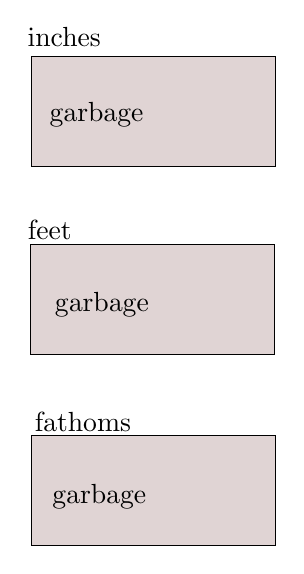
\begin{tikzpicture}[even odd rule]
\pgftransformxscale{1.000000}
\pgftransformyscale{-1.000000}
\definecolor{dialinecolor}{rgb}{0.000000, 0.000000, 0.000000}
\pgfsetstrokecolor{dialinecolor}
\pgfsetstrokeopacity{1.000000}
\definecolor{diafillcolor}{rgb}{1.000000, 1.000000, 1.000000}
\pgfsetfillcolor{diafillcolor}
\pgfsetfillopacity{1.000000}
\pgfsetlinewidth{0.020000\du}
\pgfsetdash{}{0pt}
\pgfsetmiterjoin
\pgfsetbuttcap
{\pgfsetcornersarced{\pgfpoint{0.000000\du}{0.000000\du}}\definecolor{diafillcolor}{rgb}{0.878431, 0.831373, 0.831373}
\pgfsetfillcolor{diafillcolor}
\pgfsetfillopacity{1.000000}
\fill (12.449997\du,2.411770\du)--(12.449997\du,3.811770\du)--(15.549997\du,3.811770\du)--(15.549997\du,2.411770\du)--cycle;
}{\pgfsetcornersarced{\pgfpoint{0.000000\du}{0.000000\du}}\definecolor{dialinecolor}{rgb}{0.000000, 0.000000, 0.000000}
\pgfsetstrokecolor{dialinecolor}
\pgfsetstrokeopacity{1.000000}
\draw (12.449997\du,2.411770\du)--(12.449997\du,3.811770\du)--(15.549997\du,3.811770\du)--(15.549997\du,2.411770\du)--cycle;
}% setfont left to latex
\definecolor{dialinecolor}{rgb}{0.000000, 0.000000, 0.000000}
\pgfsetstrokecolor{dialinecolor}
\pgfsetstrokeopacity{1.000000}
\definecolor{diafillcolor}{rgb}{0.000000, 0.000000, 0.000000}
\pgfsetfillcolor{diafillcolor}
\pgfsetfillopacity{1.000000}
\node[anchor=base west,inner sep=0pt,outer sep=0pt,color=dialinecolor] at (12.405000\du,2.300000\du){inches};
% setfont left to latex
\definecolor{dialinecolor}{rgb}{0.000000, 0.000000, 0.000000}
\pgfsetstrokecolor{dialinecolor}
\pgfsetstrokeopacity{1.000000}
\definecolor{diafillcolor}{rgb}{0.000000, 0.000000, 0.000000}
\pgfsetfillcolor{diafillcolor}
\pgfsetfillopacity{1.000000}
\node[anchor=base west,inner sep=0pt,outer sep=0pt,color=dialinecolor] at (12.683330\du,3.245103\du){garbage};
\pgfsetlinewidth{0.020000\du}
\pgfsetdash{}{0pt}
\pgfsetmiterjoin
\pgfsetbuttcap
{\pgfsetcornersarced{\pgfpoint{0.000000\du}{0.000000\du}}\definecolor{diafillcolor}{rgb}{0.878431, 0.831373, 0.831373}
\pgfsetfillcolor{diafillcolor}
\pgfsetfillopacity{1.000000}
\fill (12.451667\du,7.230000\du)--(12.451667\du,8.630000\du)--(15.551667\du,8.630000\du)--(15.551667\du,7.230000\du)--cycle;
}{\pgfsetcornersarced{\pgfpoint{0.000000\du}{0.000000\du}}\definecolor{dialinecolor}{rgb}{0.000000, 0.000000, 0.000000}
\pgfsetstrokecolor{dialinecolor}
\pgfsetstrokeopacity{1.000000}
\draw (12.451667\du,7.230000\du)--(12.451667\du,8.630000\du)--(15.551667\du,8.630000\du)--(15.551667\du,7.230000\du)--cycle;
}\pgfsetlinewidth{0.020000\du}
\pgfsetdash{}{0pt}
\pgfsetmiterjoin
\pgfsetbuttcap
{\pgfsetcornersarced{\pgfpoint{0.000000\du}{0.000000\du}}\definecolor{diafillcolor}{rgb}{0.878431, 0.831373, 0.831373}
\pgfsetfillcolor{diafillcolor}
\pgfsetfillopacity{1.000000}
\fill (12.435000\du,4.805000\du)--(12.435000\du,6.205000\du)--(15.535000\du,6.205000\du)--(15.535000\du,4.805000\du)--cycle;
}{\pgfsetcornersarced{\pgfpoint{0.000000\du}{0.000000\du}}\definecolor{dialinecolor}{rgb}{0.000000, 0.000000, 0.000000}
\pgfsetstrokecolor{dialinecolor}
\pgfsetstrokeopacity{1.000000}
\draw (12.435000\du,4.805000\du)--(12.435000\du,6.205000\du)--(15.535000\du,6.205000\du)--(15.535000\du,4.805000\du)--cycle;
}% setfont left to latex
\definecolor{dialinecolor}{rgb}{0.000000, 0.000000, 0.000000}
\pgfsetstrokecolor{dialinecolor}
\pgfsetstrokeopacity{1.000000}
\definecolor{diafillcolor}{rgb}{0.000000, 0.000000, 0.000000}
\pgfsetfillcolor{diafillcolor}
\pgfsetfillopacity{1.000000}
\node[anchor=base west,inner sep=0pt,outer sep=0pt,color=dialinecolor] at (12.408333\du,4.749859\du){feet};
% setfont left to latex
\definecolor{dialinecolor}{rgb}{0.000000, 0.000000, 0.000000}
\pgfsetstrokecolor{dialinecolor}
\pgfsetstrokeopacity{1.000000}
\definecolor{diafillcolor}{rgb}{0.000000, 0.000000, 0.000000}
\pgfsetfillcolor{diafillcolor}
\pgfsetfillopacity{1.000000}
\node[anchor=base west,inner sep=0pt,outer sep=0pt,color=dialinecolor] at (12.495000\du,7.186526\du){fathoms};
% setfont left to latex
\definecolor{dialinecolor}{rgb}{0.000000, 0.000000, 0.000000}
\pgfsetstrokecolor{dialinecolor}
\pgfsetstrokeopacity{1.000000}
\definecolor{diafillcolor}{rgb}{0.000000, 0.000000, 0.000000}
\pgfsetfillcolor{diafillcolor}
\pgfsetfillopacity{1.000000}
\node[anchor=base west,inner sep=0pt,outer sep=0pt,color=dialinecolor] at (12.751667\du,5.663333\du){garbage};
% setfont left to latex
\definecolor{dialinecolor}{rgb}{0.000000, 0.000000, 0.000000}
\pgfsetstrokecolor{dialinecolor}
\pgfsetstrokeopacity{1.000000}
\definecolor{diafillcolor}{rgb}{0.000000, 0.000000, 0.000000}
\pgfsetfillcolor{diafillcolor}
\pgfsetfillopacity{1.000000}
\node[anchor=base west,inner sep=0pt,outer sep=0pt,color=dialinecolor] at (12.718333\du,8.105000\du){garbage};
\end{tikzpicture}

            }
            \only<2> {
                % Graphic for TeX using PGF
% Title: /home/rjzak/Desktop/cmsc104/L07_assignment_2.dia
% Creator: Dia v0.97+git
% CreationDate: Wed Sep 22 22:57:37 2021
% For: rjzak
% \usepackage{tikz}
% The following commands are not supported in PSTricks at present
% We define them conditionally, so when they are implemented,
% this pgf file will use them.
\ifx\du\undefined
  \newlength{\du}
\fi
\setlength{\du}{15\unitlength}
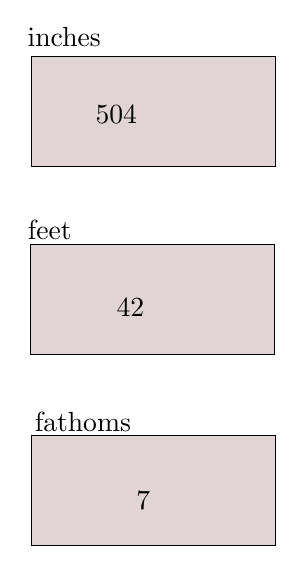
\begin{tikzpicture}[even odd rule]
\pgftransformxscale{1.000000}
\pgftransformyscale{-1.000000}
\definecolor{dialinecolor}{rgb}{0.000000, 0.000000, 0.000000}
\pgfsetstrokecolor{dialinecolor}
\pgfsetstrokeopacity{1.000000}
\definecolor{diafillcolor}{rgb}{1.000000, 1.000000, 1.000000}
\pgfsetfillcolor{diafillcolor}
\pgfsetfillopacity{1.000000}
\pgfsetlinewidth{0.020000\du}
\pgfsetdash{}{0pt}
\pgfsetmiterjoin
\pgfsetbuttcap
{\pgfsetcornersarced{\pgfpoint{0.000000\du}{0.000000\du}}\definecolor{diafillcolor}{rgb}{0.878431, 0.831373, 0.831373}
\pgfsetfillcolor{diafillcolor}
\pgfsetfillopacity{1.000000}
\fill (12.449997\du,2.411770\du)--(12.449997\du,3.811770\du)--(15.549997\du,3.811770\du)--(15.549997\du,2.411770\du)--cycle;
}{\pgfsetcornersarced{\pgfpoint{0.000000\du}{0.000000\du}}\definecolor{dialinecolor}{rgb}{0.000000, 0.000000, 0.000000}
\pgfsetstrokecolor{dialinecolor}
\pgfsetstrokeopacity{1.000000}
\draw (12.449997\du,2.411770\du)--(12.449997\du,3.811770\du)--(15.549997\du,3.811770\du)--(15.549997\du,2.411770\du)--cycle;
}% setfont left to latex
\definecolor{dialinecolor}{rgb}{0.000000, 0.000000, 0.000000}
\pgfsetstrokecolor{dialinecolor}
\pgfsetstrokeopacity{1.000000}
\definecolor{diafillcolor}{rgb}{0.000000, 0.000000, 0.000000}
\pgfsetfillcolor{diafillcolor}
\pgfsetfillopacity{1.000000}
\node[anchor=base west,inner sep=0pt,outer sep=0pt,color=dialinecolor] at (12.405000\du,2.300000\du){inches};
% setfont left to latex
\definecolor{dialinecolor}{rgb}{0.000000, 0.000000, 0.000000}
\pgfsetstrokecolor{dialinecolor}
\pgfsetstrokeopacity{1.000000}
\definecolor{diafillcolor}{rgb}{0.000000, 0.000000, 0.000000}
\pgfsetfillcolor{diafillcolor}
\pgfsetfillopacity{1.000000}
\node[anchor=base west,inner sep=0pt,outer sep=0pt,color=dialinecolor] at (13.266663\du,3.278437\du){504};
\pgfsetlinewidth{0.020000\du}
\pgfsetdash{}{0pt}
\pgfsetmiterjoin
\pgfsetbuttcap
{\pgfsetcornersarced{\pgfpoint{0.000000\du}{0.000000\du}}\definecolor{diafillcolor}{rgb}{0.878431, 0.831373, 0.831373}
\pgfsetfillcolor{diafillcolor}
\pgfsetfillopacity{1.000000}
\fill (12.451667\du,7.230000\du)--(12.451667\du,8.630000\du)--(15.551667\du,8.630000\du)--(15.551667\du,7.230000\du)--cycle;
}{\pgfsetcornersarced{\pgfpoint{0.000000\du}{0.000000\du}}\definecolor{dialinecolor}{rgb}{0.000000, 0.000000, 0.000000}
\pgfsetstrokecolor{dialinecolor}
\pgfsetstrokeopacity{1.000000}
\draw (12.451667\du,7.230000\du)--(12.451667\du,8.630000\du)--(15.551667\du,8.630000\du)--(15.551667\du,7.230000\du)--cycle;
}\pgfsetlinewidth{0.020000\du}
\pgfsetdash{}{0pt}
\pgfsetmiterjoin
\pgfsetbuttcap
{\pgfsetcornersarced{\pgfpoint{0.000000\du}{0.000000\du}}\definecolor{diafillcolor}{rgb}{0.878431, 0.831373, 0.831373}
\pgfsetfillcolor{diafillcolor}
\pgfsetfillopacity{1.000000}
\fill (12.435000\du,4.805000\du)--(12.435000\du,6.205000\du)--(15.535000\du,6.205000\du)--(15.535000\du,4.805000\du)--cycle;
}{\pgfsetcornersarced{\pgfpoint{0.000000\du}{0.000000\du}}\definecolor{dialinecolor}{rgb}{0.000000, 0.000000, 0.000000}
\pgfsetstrokecolor{dialinecolor}
\pgfsetstrokeopacity{1.000000}
\draw (12.435000\du,4.805000\du)--(12.435000\du,6.205000\du)--(15.535000\du,6.205000\du)--(15.535000\du,4.805000\du)--cycle;
}% setfont left to latex
\definecolor{dialinecolor}{rgb}{0.000000, 0.000000, 0.000000}
\pgfsetstrokecolor{dialinecolor}
\pgfsetstrokeopacity{1.000000}
\definecolor{diafillcolor}{rgb}{0.000000, 0.000000, 0.000000}
\pgfsetfillcolor{diafillcolor}
\pgfsetfillopacity{1.000000}
\node[anchor=base west,inner sep=0pt,outer sep=0pt,color=dialinecolor] at (12.408333\du,4.749859\du){feet};
% setfont left to latex
\definecolor{dialinecolor}{rgb}{0.000000, 0.000000, 0.000000}
\pgfsetstrokecolor{dialinecolor}
\pgfsetstrokeopacity{1.000000}
\definecolor{diafillcolor}{rgb}{0.000000, 0.000000, 0.000000}
\pgfsetfillcolor{diafillcolor}
\pgfsetfillopacity{1.000000}
\node[anchor=base west,inner sep=0pt,outer sep=0pt,color=dialinecolor] at (12.495000\du,7.186526\du){fathoms};
% setfont left to latex
\definecolor{dialinecolor}{rgb}{0.000000, 0.000000, 0.000000}
\pgfsetstrokecolor{dialinecolor}
\pgfsetstrokeopacity{1.000000}
\definecolor{diafillcolor}{rgb}{0.000000, 0.000000, 0.000000}
\pgfsetfillcolor{diafillcolor}
\pgfsetfillopacity{1.000000}
\node[anchor=base west,inner sep=0pt,outer sep=0pt,color=dialinecolor] at (13.535000\du,5.730000\du){42};
% setfont left to latex
\definecolor{dialinecolor}{rgb}{0.000000, 0.000000, 0.000000}
\pgfsetstrokecolor{dialinecolor}
\pgfsetstrokeopacity{1.000000}
\definecolor{diafillcolor}{rgb}{0.000000, 0.000000, 0.000000}
\pgfsetfillcolor{diafillcolor}
\pgfsetfillopacity{1.000000}
\node[anchor=base west,inner sep=0pt,outer sep=0pt,color=dialinecolor] at (13.785000\du,8.171667\du){7};
\end{tikzpicture}

            }
    \end{columns}
\end{frame}

\begin{frame}{Enhancing the Example}
    \begin{itemize}
        \item What if the depth was really 6.75 fathoms? Our program, as is, couldn't handle it.
        \item Unlike integers, floating point numbers can contain numbers after the decimal point.
        \item Let's also ask the user for input instead of \textbf{hard-coding} values in the program.
    \end{itemize}
\end{frame}

\begin{frame}[fragile]{Enhanced Program}
\begin{lstlisting}[language=C,basicstyle=\footnotesize,keywordstyle=\color{blue},commentstyle=\color{green},showstringspaces=false,stringstyle=\color{red}]
    #include <stdio.h>
    int main() {
        float inches, feet, fathoms;
        printf("Enter the depth in fathoms: ");
        scanf("%f", &fathoms);
        feet = 6.0 * fathoms;
        inches = 12.0 * feet;
        printf("Its depth at sea:\n");
        printf("\t%1.2f fathoms\n", fathoms);
        printf("\t%1.2f feet\n", feet);
        printf("\t%1.2f inches\n", inches);
        return 0;
    }
\end{lstlisting}
\end{frame}

\begin{frame}[fragile]{Final ``Clean'' Program}
\begin{lstlisting}[language=C,basicstyle=\footnotesize,keywordstyle=\color{blue},commentstyle=\color{green},showstringspaces=false,stringstyle=\color{red}]
    #include <stdio.h>
    int main() {
        float inches;  /* number of inches deep */
        float feet;    /* number of feet deep */
        float fathoms; /* number of fathoms deep */
        
        /* Ask the user for the depth */
        printf("Enter the depth in fathoms: ");
        scanf("%f", &fathoms);
        
        /* Convert depth from fathoms to inches */
        feet = 6.0 * fathoms;
        inches = 12.0 * feet;
        
        /* Display the results */
        printf("Its depth at sea:\n");
        printf("\t%1.2f fathoms\n", fathoms);
        printf("\t%1.2f feet\n", feet);
        printf("\t%1.2f inches\n", inches);
        return 0;
    }
\end{lstlisting}
\end{frame}

\begin{frame}{Good Programming Practices}
    \begin{itemize}
        \item Place a comment before each logical ``chunk'' of code describing what it does.
        \item Do not place a comment on the same line as code (with the exception of variable declarations).
        \item Use spaces around all assignment and arithmetic operators.
        \item Use blank lines to enhance readability.
        \item Place a blank line between the last variable declaration and first executable statement of the program.
        \item Indent the body of the program three or four spaces -- be consistent!
    \end{itemize}
\end{frame}

\end{document}